\begin{figure}[h!]
    \centering
    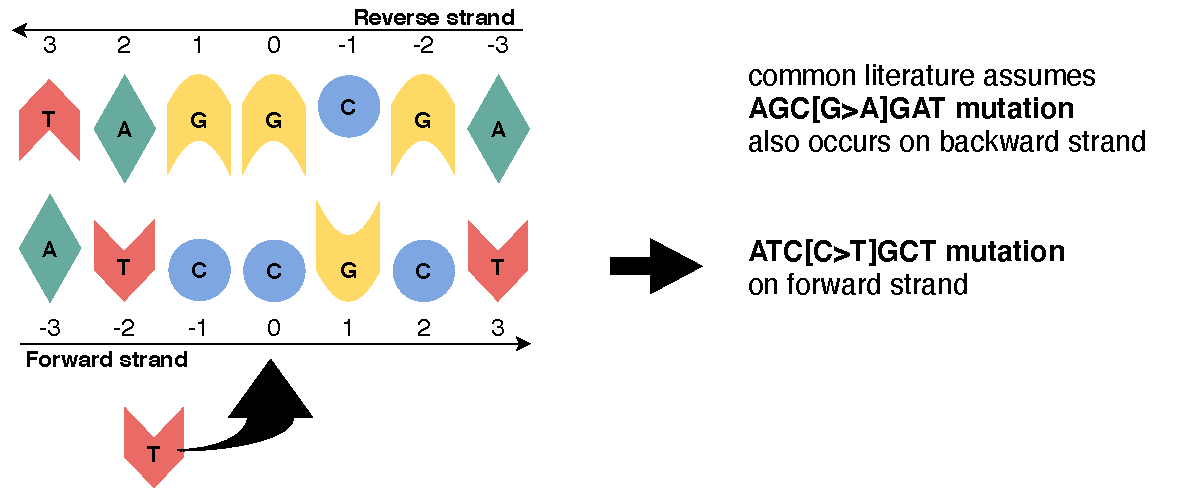
\includegraphics[scale=0.78]{graphics/motif_symmetric_demo.pdf}
    \caption{\textbf{It is common practice to assume strand symmetry when analysing mutations.} In this example, AGC[G$\rightarrow$A]GAT and ATC[C$\rightarrow$G]GCT mutation on the reverse complementary strand are counted as the same category. However, observations supporting strand asymmetry have been reported. This project explores the effect of the strand symmetric \textit{v.s.} strand asymmetric assumption.}
    \label{fig:motif_symmetric_demo}
\end{figure}
